\section{Principal Component Analysis}  

  Say that we have a random vector $x = (x_1, \ldots, x_d)$. These $d$ covariates will naturally be correlated, and we want to ask whether some more fundamental set of independent variables exist \cite{1933hotelling} such that we can express
  \begin{equation}
    x = f(v_1, \ldots, v_k)
  \end{equation} 
  Naturally, we think of $f$ as a linear function. 

  We can think of PCA doing two things. First, it is a dimensionality-reduction algorithm where it takes samples $x \in \mathbb{R}^d$ and projects them into some smaller subspace $\mathcal{L}$ of dimension $k$. Second, it identifies an orthonormal basis of $\mathcal{L}$ that act as uncorrelated low-dimensional features. Because the projection map is linear and we are working in a lower-dimensional subspace, these new basis vectors are linear combinations of the original basis, which may reduce redundancy. Furthermore, by approximately modeling the original $x$ as a linear combination of these features, we are able to get a more parsimonious representation. 

  In PCA literature, it is more common to work with row vectors $x \in \mathbb{R}^{1 \times d}$, so linear mappings are realized through right matrix multiplication $x A$. Furthermore, we will assume that the data are $0$-mean. 

\subsection{L2 Residual Minimization Approach} 

  To give some motivation, we try to find a best fit line in $\mathbb{R}^d$. A line $\ell$ can be parameterized by a unit vector $v$, and so given some sample $x$, its projection onto $\ell$ is $\proj_{\ell} (x) = \langle x, v\rangle v$. Therefore, the residual is 
  \begin{align}
    \| x - \langle x, v \rangle v \|^2 & = \|x\|^2 - 2 \langle x, \langle x, v \rangle v \rangle + \| \langle x, v \rangle v \|^2 \\ 
                                       & = \|x\|^2 - 2 \langle x, v \rangle^2 + \langle x, v \rangle^2 \|v\|^2 \\ 
                                       & = \|x\|^2 - \langle x, v \rangle^2
  \end{align}
  since $\|v\|^2 = 1$ \cite{2019shalizi}. 

  Now given a random variable $x$, our risk is
  \begin{equation}
    R(v) = \mathbb{E}_x \big[ \| x - (x \cdot v) v \| \big] = \mathbb{E}_x \big[ \|x\|^2 \big] - \mathbb{E}_x \big[ \langle x, v \rangle^2 \big]
  \end{equation} 

  In practice, we want to minimize our empirical risk. Assume that we have sampled data $x^{(1)}, \ldots, x^{(n)} \sim x$. Then, 
  \begin{align} 
    \argmin_{v \in \mathbb{R}^{d}, \|v\| = 1} \hat{R}(v) 
    & =  \argmin_{v \in \mathbb{R}^{d}, \|v\| = 1} \frac{1}{n} \bigg( \sum_{i = 1}^n \|x^{(i)} \|^2 - \sum_{i=1}^n \langle x^{(i)}, v \rangle^2 \bigg) \\ 
    & = \argmax_{v \in \mathbb{R}^{d}, \|v\| = 1} \frac{1}{n} \sum_{i=1}^n \langle x^{(i)}, v \rangle^2 
  \end{align} 

  We have our loss function! Now what if we wanted to look for best fitting subspaces in general? Let's first rigorously define such a space. 

  \begin{definition}[Principal Subspace] 
    Let $x$ be a $0$-mean random variable in $\mathbb{R}^d$ and let $\mathcal{L}^k$ denote all $k$-dimensional linear subspaces of $\mathbb{R}^d$. The \textbf{$k$th principal subspace} is defined as 
    \begin{equation}
      \ell_k = \argmin_{\ell \in \mathcal{L}_k} \mathbb{E}_{\Tilde{x}} \big[ \| x - \proj_\ell x\|_2 \big]
    \end{equation}
  \end{definition}

  This isn't a big step from what we had before. We just want to construct a subspace $\ell$ that minimizes the expected $L^2$ distance between $x$ and $\ell$. Now how do we do such a thing? The most natural extension would be to identify an orthonormal basis $v_1, \ldots, v_k$, and since 
  \begin{equation}
    \proj_\ell x = \sum_{i=1}^k \proj_{v_i} x
  \end{equation} 
  our loss can be simplified to 
  \begin{align}
    R(\ell) = R(v_1, \ldots, v_k) 
    & = \mathbb{E} \bigg[ \| x - \proj_\ell x \|^2 \bigg] \\ 
    & = \mathbb{E} \bigg[ \|x\|^2 - 2 \langle x, \sum_{i=1}^k \proj_{v_i} x \rangle + \| \sum_{i=1}^k \proj_{v_i} x \|^2 \bigg] \\ 
    & = \mathbb{E} \bigg[ \|x\|^2 - 2 \sum_{i=1}^k \langle x, \proj_{v_i} x \rangle + \sum_{i=1}^k \| \proj_{v_i} x \|^2 \bigg] \\
    & = \mathbb{E} \bigg[ \|x\|^2 - 2 \sum_{i=1}^k \langle x, v_i \rangle^2 + \sum_{i=1}^k \langle x, v_i \rangle^2 \|v_i\|^2 \bigg] \\ 
    & = \mathbb{E} \bigg[ \|x\|^2 - \sum_{i=1}^k \langle x, v_i \rangle^2 \bigg] 
  \end{align} 
  and in the empirical case, we can get rid of the fixed $x$ and find 
  \begin{equation}
    \argmax_{v_i \in \mathbb{R}^d} \frac{1}{n} \sum_{j=1}^n \sum_{i=1}^k \langle x^{(j)}, v_i \rangle^2, \quad \text{ subject to } \|v_i\|^2 = 1, \langle v_i, v_j \rangle = 0 \text{ for } i \neq j
  \end{equation} 

  By stacking the $v_i$'s left-to-right in matrix $V_k \in \mathbb{R}^{d \times k}$, we can get a cleaner form of the loss function. 
  \begin{align}
    \frac{1}{n} \sum_{j=1}^n \sum_{i=1}^k \langle x^{(j)}, v_i \rangle^2 
    & = \frac{1}{n} \sum_{j=1}^n \sum_{i=1}^k (x^{(j)})^T v_i v_i^T x^{(j)} \\ 
    & = \frac{1}{n} \sum_{j=1}^n (x^{(j)})^T V_k V_k^T x^{(j)} \\ 
    & = \frac{1}{n} \Tr(X V_k V_k^T X^T) = \frac{1}{n} \Tr(V_k^T X^T  X V_k) \label{trace}
  \end{align}
  This leads to an intuitive loss function for PCA. 

  \begin{theorem}[Constrained Empirical Risk of $k$th Principal Subspace]
    The empirical risk, or loss function, of PCA is
    \begin{equation}
      \argmax_{V \in \mathbb{R}^{d \times k}, V_k^T V_k = I_k} 
      \frac{1}{n} \| X - X V_k V_k^T\|^2
    \end{equation}
  \end{theorem} 
  \begin{proof}
    By the Frobenius norm expansion and since $V_k^T V_k = I_k$, we have 
    \begin{align}
      \|X - X V_k V_k^T\|_F^2 
      & = \Tr((X - X V_k V_k^T)^T(X - X V_k V_k^T)) \\
      & = \Tr(X^T X - X^T X V_k V_k^T - V_k V_k^T X^T X + V_k V_k^T X^T X V_k V_k^T) \\
      & = \Tr(X^T X) - 2\Tr(X^T X V_k V_k^T) + \Tr(V_k V_k^T X^T X V_k V_k^T) \\ 
      & = \Tr(X^T X) - 2\Tr(V_k^T X^T X V_k) + \Tr(V_k^T V_k V_k^T X^T X V_k) \\
      & = \Tr(X^T X) - 2\Tr(V_k^T X^T X V_k) + \Tr(V_k^T X^T X V_k) \\ 
      & = \Tr(X^T X) - \Tr(V_k^T X^T X V_k) 
    \end{align}
    and since the empirical risk does not depend on $X$, minimizing the Frobenius norm is equivalent to maximizing the second trace term, i.e. \ref{trace}. 
  \end{proof}

  \begin{definition}[Projection Operator]
    Note that there are two distinct projection operators, which are realized through right matrix multiplication. 
    \begin{enumerate}
      \item The linear map $V_k : \mathbb{R}^d \to \mathbb{R}^k$ is a projection operator of the samples $x$ into the component space. 
      \item The linear map $V_k V_k^T : \mathbb{R}^d \to \mathbb{R}^d$ is called the \textbf{rank-k projection operator} onto the $k$th principal subspace. 
    \end{enumerate}
  \end{definition}

  Therefore, $X V_k \in \mathbb{R}^{n \times k}$ is the projection of the dataset into the component space. If we want to get the denoised samples in the sample space $\mathbb{R}^d$, we project it back out $X V_k V_k^T$. 

\subsection{Variance Maximization Approach}

  But we can turn this into a variance maximization problem. Note that $\Var_x [\langle x, v \rangle] = \mathbb{E}_x [ \langle x, v \rangle^2 ] - \mathbb{E}_x [ \langle x, v \rangle]^2$, and so we can rewrite our true risk as 
  \begin{align}
    \argmin_{v \in \mathbb{R}^d, \|v\|=1} R(v) = \argmin_{v \in \mathbb{R}^d, \|v\|=1} \mathbb{E}_x \big[ \|x\|^2 \big] - \Var_x [\langle x, v \rangle] - \mathbb{E}_x [ \langle x, v \rangle]^2
  \end{align} 
  where the last term vanishes since $x$ is $0$-mean, and hence by linearity of expectation $\mathbb{E}_x [\langle x, v \rangle] = \langle \mathbb{E}[x], v \rangle = \langle 0, v \rangle = 0$. In parallel the empirical risk reduces to simply the sample variance. 
  \begin{equation}
    \argmax_{v \in \mathbb{R}^{d}, \|v\| = 1} \hat{\Var}[ \langle x, v \rangle] = \argmax_{v \in \mathbb{R}^{d}, \|v\| = 1} \frac{1}{n} \bigg( \sum_{i=1}^n \langle x^{(i)}, v \rangle^2 \bigg)
  \end{equation} 

  Therefore, we can think of the $L^2$ minimization problem as equivalent to a variance maximization approach.  

  \begin{lemma}[Variance Maximization Approach]
    Minimizing the $L^2$ distance of a random variable $x$ to a line $\ell$ in $\mathbb{R}^d$ is equivalent to maximizing the scalar variance in the projected space. 
    \begin{equation}
      \argmin_{v \in \mathbb{R}^d, \|v\| = 1} \mathbb{E} [ \| x - \proj_v (x) \|_2 ] = \argmax_{v \in \mathbb{R}^d, \|v\| = 1} \Var_x [\langle x, v \rangle ]
    \end{equation}
  \end{lemma}

  \begin{figure}[H]
    \centering
    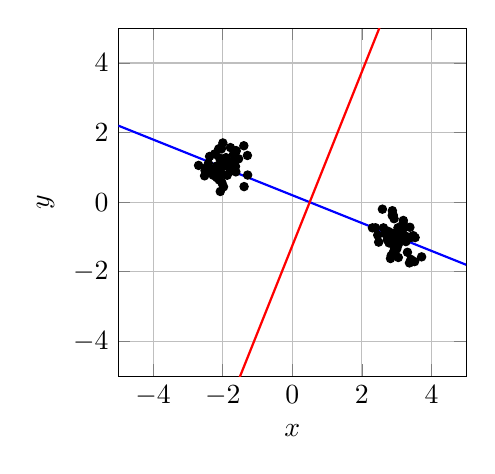
\begin{tikzpicture}
      \begin{axis}[
        xlabel={$x$}, ylabel={$y$},
        axis equal,
        xmin=-5, xmax=5,
        ymin=-5, ymax=5,
        grid=both,
        width=6cm, height=6cm
      ]
      
      \foreach \i in {1,...,50} {
        \pgfmathsetmacro\x{-2 + 0.8*rnd*cos(360*rnd)}
        \pgfmathsetmacro\y{1 + 0.8*rnd*sin(360*rnd)}
        \addplot[only marks, mark=*, mark size=1.5pt, color=black] coordinates {(\x,\y)};
      }
      
      \foreach \i in {1,...,50} {
        \pgfmathsetmacro\x{3 + 0.8*rnd*cos(360*rnd)}
        \pgfmathsetmacro\y{-1 + 0.8*rnd*sin(360*rnd)}
        \addplot[only marks, mark=*, mark size=1.5pt, color=black] coordinates {(\x,\y)};
      }

      % Line from (-2,1) to (3,-1): slope -2/5
      \addplot[thick, blue, domain=-5:5, samples=2] {-0.4*(x + 2) + 1};

      % Perpendicular line through midpoint (0.5, 0), slope 5/2
      \addplot[thick, red, domain=-5:5, samples=2] {2.5*(x - 0.5)};
      \end{axis}
    \end{tikzpicture}
    \caption{Projecting the dataset onto the blue line seems to retain more variance than projecting onto the red line.}
  \end{figure}

  Let's in fact try to directly maximize the variance. If we vertically stack our $n$ data points into a matrix $X \in \mathbb{R}^{n \times d}$, then the projections of this data onto $\mathbb{R}$ is simply $X v \in \mathbb{R}^n$. Again, since this is $0$-mean, the variance is 
  \begin{align}
    \label{eq:var_decom}
    \hat{\Var}(Xv) 
    & = \frac{1}{n} (Xv)^T (Xv) \\ 
    & = \frac{1}{n} v^T X^T X v \\
    & = v^T \frac{X^T X}{n} v \\ 
    & = v^T \hat{\Sigma} v
  \end{align}
  where $\hat{\Sigma}$ is the empirical covariance matrix of $X$. We want to find 
  \begin{equation}
    \max_{v} v^T \hat{\Sigma} v \text{ subject to } \|v\|^2 = 1
  \end{equation} 
  This is a classic Lagrange multiplier problem. We construct the Lagrangian and compute its partial derivatives to set equal to $0$. 
  \begin{align}
    \mathcal{L}(v, \lambda) & = v^T \hat{\Sigma} v - \lambda (\|v\|^2 - 1) \\  
    \frac{\partial \mathcal{L}}{\partial v} & = 2 \hat{\Sigma} v - 2 \lambda v = 0 \\ 
    \frac{\partial \mathcal{L}}{\partial \lambda} & = v^T v - 1 = 0
  \end{align} 
  which gives us 
  \begin{equation}
    \hat{\Sigma} v = \lambda v, \qquad v^T v = 1
  \end{equation} 
  This tells us that $v$ is a unit eigenvector, and the maximizing vector will be the one corresponding to the largest eigenvalue. Essentially, we have reduced this to an eigenvalue problem. 
  
  \begin{theorem}[1st Principal Subspace as Eigenvector]
    The first principal subspace of data matrix $X \in \mathbb{R}^{n \times d}$ is spanned by the eigenvector corresponding to the largest eigenvalue of the sample covariance matrix $\hat{\Sigma} = \frac{1}{n} X^T X$. 
  \end{theorem}

  Now for higher dimensional subspaces, we take the same approach. Going through the same derivation gives the expected risk in terms of the variance 
  \begin{align}
    R(v_1, \ldots, v_k) 
    & = \mathbb{E}[\|x\|^2] - \sum_{i=1}^k \mathbb{E}[ \langle x, v_i \rangle^2 ] \\ 
    & = \mathbb{E}[\|x\|^2] - \sum_{i=1}^k \Var[\langle x, v_i \rangle ] - \mathbb{E}[ \langle x, v_i \rangle ]^2 
  \end{align} 
  By fixing the $x$'s and going through the same derivation as \ref{eq:var_decom}, we get our equivalent empirical risk. 
  \begin{equation}
    \argmax_{v_i \in \mathbb{R}^d} \sum_{i=1}^k \hat{\Var}[\langle x, v_i \rangle] = \argmax_{v_i \in \mathbb{R}^d} \sum_{i=1}^k v_i^T \hat{\Sigma} v_i
  \end{equation}

  \begin{theorem}[Constrained Empirical Risk of $k$th Principal Subspace]
    The empirical risk tells us to find an orthonormal basis that maximizes the sum of the variance of projections. 
    \begin{equation}
      \argmax_{v_i \in \mathbb{R}^d} \sum_{i=1}^k  v_i^T \hat{\Sigma} v_i \text{ subject to } \|v_i\|^2 = 1, \langle v_i, v_j \rangle = 0 \text{ for } i \neq j
    \end{equation}
  \end{theorem}

  The variance-maximization loss is very insightful, and we may naively think of just taking the unit eigenvectors corresponding to the top $k$ largest eigenvalues. Surprisingly, this greedy approach turns out to be correct. 

  Let's derive this further 
  \begin{align}
    \sum_{i = 1}^k v_i^T \hat{\Sigma} v_i 
    & = \sum_{i=1}^k \Tr(v_i v_i^T \hat{\Sigma}) \\ 
    & = \Tr(V_k V_k^T \hat{\Sigma}) \\ 
    & = \Tr(\hat{\Sigma} V_k V_k^T)
  \end{align}
  which again is equal to \ref{trace}. By the spectral theorem, we can take the eigendecomposition of self-adjoint $\hat{\Sigma} = Q \Lambda Q^T$ with orthogonal matrix $Q$. Setting $W_k = Q^T V_k$, we have 
  \begin{equation}
    \Tr(\hat{\Sigma} V_k V_k^T) = \Tr(Q \Lambda Q^T V_k V_k^T) = \Tr(\Lambda Q^T V_k V_k^T Q) = \Tr(\Lambda W_k W_k^T) = \sum_{i = 1}^d \lambda_i (W_k W_k^T)_{ii}
  \end{equation}
  where without loss of generality we have $\lambda_1 \geq \lambda_2 \geq \ldots \geq \lambda_d$. However, we have two constraints. First, since $W_k W_k^T$ is a projection matrix, the eigenvalues must be between $0$ and $1$. Second, by the cyclic trace property, we have $\Tr(W_k W_k^T) = \Tr(I_k) = k$.\footnote{Though it is \textit{not} the case that $W_k W_k^T = I_k$!} So denoting $w_i = (W_k W_k^T)_{ii}$, we have the optimal allocation problem 
  \begin{equation}
    \max \sum_{i=1}^d \lambda_i w_i \text{ subject to } \begin{cases} 
      w_i \in [0, 1] \; \forall i = 1, \ldots, d \\
      \sum_i w_i = k
    \end{cases}
  \end{equation}
  Since the eigenvalues are decreasing, it doesn't take too much to see that the optimal solution is to just put everything you have into the largest eigenvalues. So we fill the first $w_1 = \ldots = w_k = 1$ and the rest $w_{k+1}, \ldots w_d = 0$. Therefore, this solution corresponds to $W_k = (e_1, e_2, \ldots, e_k)$, and so 
  \begin{equation}
    V_k = Q W_k = Q_k
  \end{equation}
  which is the truncated matrix $Q$ containing the first $k$ eigenvectors of $\hat{\Sigma}$ corresponding to the largest eigenvalues. At this point, it does not suffice to talk about just a principal subspace anymore. We must identify its orthonormal basis, i.e. the eigenvectors. 

  \begin{definition}[Principal Axis]
    The eigenvectors $v_1, \ldots, v_k$ that span the $k$th principal subspace are called the top $k$ \textbf{principal axes}, or \textbf{principal directions}.\footnote{The terminology is misused and confusing sometimes. See \href{https://stats.stackexchange.com/questions/88118/what-exactly-is-called-principal-component-in-pca}{https://stats.stackexchange.com/questions/88118/what-exactly-is-called-principal-component-in-pca}.} 
  \end{definition}

  This is similar to taking the first principal component $v_1$ on $X$, and then by computing the first principal component on the remaining residuals $X - \proj_{v_1} X$, we get the second principal component, which is guaranteed to be orthogonal. But usually, we end up just computing all eigenvectors at once. 

  Now how do we know that this sample decomposition is a good approximation to the true decomposition? It comes from the fact that the sample covariance $\hat{\Sigma}$ is a good approximation of the true covariance $\Sigma$, which we will later prove using concentration of measure. 

  \begin{theorem}[Risk]
    The risk satisfies 
    \begin{equation}
      R(k) = \mathbb{E}[|| x - P_k (x) ||^2 ] = \sum_{j=k+1}^D \lambda_j 
    \end{equation}
  \end{theorem}

  It is essential that you plot the spectrum in decreasing order. This allows you to analyze how well PCA is working. People often use the ``elbow'' technique to determine where to choose $K$, and we value 
  \begin{equation}
    \frac{\sum_{j=1}^k \lambda_j}{\sum_{j=1}^d \lambda_j} 
  \end{equation}
  accounts for the \textbf{variance explained}, which should be high with $K$ low. If you have to go out to dimension $K=50$ to explain $90\%$ of the variance, then PCA is not working. It may not work because of many reasons, such as there being nonlinear structure within the data. 

\subsection{Decomposition Solvers}

  \begin{theorem}[Construction of the kth Principle Subspace] 
    Let $X \in \mathbb{R}^{n \times d}$ be a $0$-mean data matrix. Given the SVD with the singular values listed in decreasing order\footnote{We can make it decreasing by permuting the rows/columns of the unitary matrices $U, V$.}
    \begin{equation}
      X = U \Sigma V^T, \qquad U \in \mathbb{R}^{n \times n}, \Sigma \in \mathbb{R}^{n \times d}, V \in \mathbb{R}^{d \times d}
    \end{equation}
  \end{theorem}

  Since $\frac{1}{n} X^T X = \frac{1}{n} V \Sigma U^T U \sigma V^T = \frac{1}{n} V \Sigma^2 V^T$, the columns of $V$ are the principal axes. Recall from linear algebra that $\Lambda = \Sigma^2$. 

  \begin{definition}[Principal Component Scores]
    The columns of $U \Sigma$ are called the \textbf{principal component scores}. 
  \end{definition}

  \begin{algo}[PCA with SVD] 
    Given a dataset $X \in \mathbb{R}^{n \times d}$, let us denote the rows as $x_i$, and say that we are looking for a subspace of dimension $k$. 
    \begin{enumerate}
      \item Compute the mean 
      \begin{equation}
        \mu = \frac{1}{n} \sum_{i=1}^n x_i  \in \mathbb{R}^d
      \end{equation} 

      \item Standardize the data $\Tilde{X} = X - \mu$, i.e. $\Tilde{x}_i = x_i - \mu$.  

      \item Compute the SVD $\Tilde{X} = U \Sigma V^T$.

      \item Compute the submatrices $V_k \in \mathbb{R}^{k \times k}$ and $\Sigma_k \in \mathbb{R}^{D \times k}$. 

      \item Define the projection operator $P_k (x) = \mu + \sum_{j=1}^k \langle x - \mu, v_j \rangle \, v_j$, the change of basis operator $T$, and the embedding operator $T^{-1} (z) = \mu + V_k \Sigma_k z$. 
    \end{enumerate} 
    A demonstration is done \href{code/pca.html}{here}.
  \end{algo}

  \begin{example}[Walkthrough]
    Say that we have some dataset of 100 points in $\mathbb{R}^3$. The data matrix is shown on the right, but in reality I just generated a toy dataset. 

    \noindent\begin{minipage}{.5\textwidth}
      \begin{lstlisting}[]{Code}
        def scatter(n=1000): 
          X_2d = np.random.multivariate_normal(
            np.zeros(2), np.eye(2), n) 
          A = np.array([[1, 1, 1], [-2, 2, 1]])
          X_3d = X_2d @ A + np.random.multivariate_normal(
            np.zeros(3), np.eye(3), n)
          return X_3d
      \end{lstlisting}
      \end{minipage}
      \hfill
      \begin{minipage}{.49\textwidth}
      \begin{lstlisting}[]{Output}
        [[ 8.864e-01  3.975e-01  7.009e-01]
         [-2.065e+00  3.258e+00  1.874e+00]
         [ 3.970e-01 -5.400e-01 -3.054e-01]
         [ 3.239e+00 -1.999e+00 -1.034e+00]
         ...
         [-1.295e-01  9.683e-01  2.861e-01]
         [-7.097e-01 -4.060e-01 -1.058e+00]
         [ 2.284e+00 -2.505e+00 -1.522e+00]]
      \end{lstlisting}
    \end{minipage}

    We can take the SVD, which will give us

    \begin{lstlisting}
      In [7]: U, S, Vt = np.linalg.svd(X)

      In [8]: print(U)
      [[ 4.804e-04  7.852e-02  4.071e-02 ...  5.320e-03  5.034e-02 -9.305e-02]
       [ 1.420e-01  3.992e-02 -1.229e-02 ... -5.512e-02  4.460e-02  7.192e-02]
       [-2.456e-02 -3.657e-03 -4.578e-04 ... -1.005e-01 -1.512e-01 -7.300e-02]
       ...
       [ 2.909e-02  2.754e-02 -1.075e-01 ...  9.871e-01 -1.325e-02 -3.559e-03]
       [-8.714e-03 -8.159e-02 -1.436e-01 ... -1.297e-02  9.733e-01 -1.055e-02]
       [-1.241e-01  2.077e-03 -6.028e-02 ... -3.435e-03 -8.286e-03  9.819e-01]]

      In [9]: print(S)
      [29.90178039 15.17454164  3.01267412]

      In [10]: print(Vt.T)
      [[-0.59855644  0.77282378 -0.21088764]
       [ 0.70716875  0.38606989 -0.59233639]
       [ 0.37635428  0.50367991  0.77760144]] 
    \end{lstlisting} 

    The \texttt{Vt.T} represents $V$, with its columns being our principal axes, and we wish to plot them along with our data points. We would like to scale them by their variance captured. 
    \begin{enumerate}
      \item Take the singular values $(\sigma_1, \sigma_2, \sigma_3) = (29.9, 15.2, 3.0)$. 
      \item Square them to get the eigenvalues $(\lambda_1, \lambda_2, \lambda_3) = (894, 230, 9)$. 
      \item Normalize them to get the percent variance captured. $(0.789, 0.203, 0.008)$, and use this as a scale for each eigenvector. 
    \end{enumerate}

    \begin{figure}[H]
      \centering 
      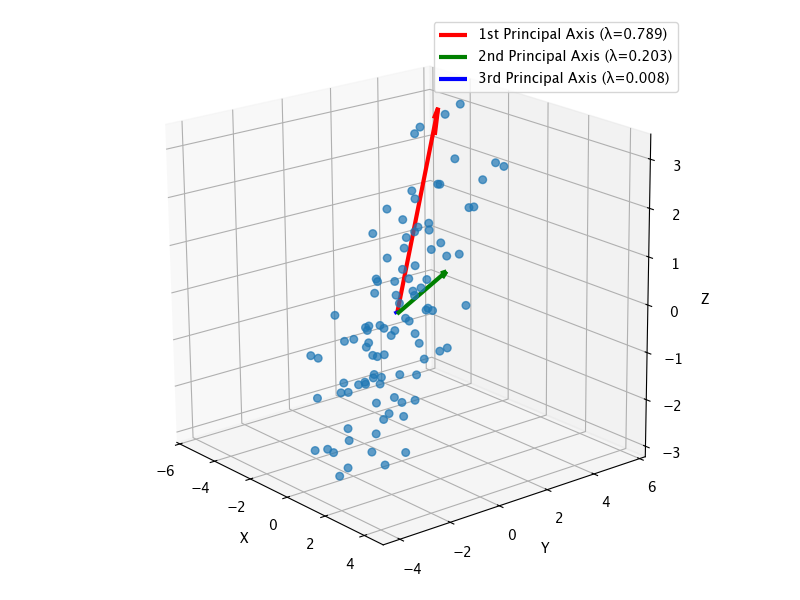
\includegraphics[scale=0.4]{img/pca_3d.png}
      \caption{We can see that the data approximately lies on a 2-dimensional subspace of $\mathbb{R}^3$.} 
    \end{figure}
  \end{example}

  \begin{example}[Eigenfaces]
    In 1991, Turk and Pentland presented an eigenface method of face recognition by taking the low-rank approximation of a dataset of face images \cite{1991turk}. 

    \begin{figure}[H]
      \centering 
      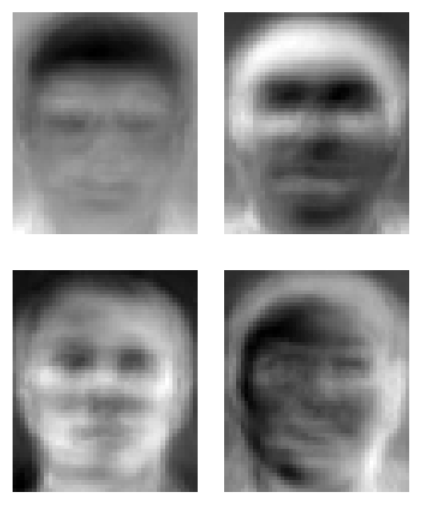
\includegraphics[scale=0.3]{img/eigenfaces.png}
      \caption{Some eigenfaces from AT\&T Labs. } 
      \label{fig:eigenfaces}
    \end{figure}
  \end{example}

\subsection{Iterative Solvers}

\subsection{The Importance of Standardizing}

\subsection{Asymptotic Analysis}

  It turns out that the elements of $\hat{\Sigma}$ are close entry-wise to those of $\Sigma$. But if this is true, then does it mean that the eigenvalues of the sample covariance matrix are close to the true eigenvalues of the covariance matrix? It turns out that the answer is no, and we need a proper metric to satisfy this assumption. The metric, as we can guess from linear algebra, is the operator norm, and we will show some results from matrix perturbation theory. 

  \begin{lemma}[]
    It turns out that 
    \begin{equation}
      ||\hat{\Sigma} - \Sigma|| = O_p \bigg( \frac{1}{\sqrt{n}} \bigg)
    \end{equation}
    where $|| \cdot ||$ is the operator norm. 
  \end{lemma}

  \begin{theorem}[Weyl's Theorem]
    If $\hat{\Sigma}$ and $\Sigma$ are close in the operator norm, then their eigenvalues are close. 
    \begin{equation}
      ||\hat{\Sigma} - \Sigma|| = O_p \bigg( \frac{1}{\sqrt{n}} \bigg) \implies |\hat{\lambda}_j - \lambda_j| = O_p \bigg( \frac{1}{\sqrt{n}} \bigg) 
    \end{equation}
  \end{theorem}

  This only talks about their eigenvalues, but this does not necessarily imply that the eigenvalues are close. We need an extra condition. 

  \begin{theorem}[David-Kahan Theorem]
    If $\hat{\Sigma}$ and $\Sigma$ are close in the operator norm, and if the eigenvectors of $\Sigma$ are well-conditioned, then the eigenvectors of $\hat{\Sigma}$ are close to the eigenvectors of $\Sigma$. More specifically, 
    \begin{equation}
      ||\hat{v}_j - v_j|| \leq \frac{2^{3/2} ||\hat{\Sigma} - \Sigma||}{\lambda_j - \lambda_{j+1}}
    \end{equation}
  \end{theorem}



